\documentclass[10pt,a4paper]{article}

% ================================================================
% PREMIUM TWO-PAGE LATEX PORTFOLIO
% ================================================================
\usepackage[T1]{fontenc}
\usepackage[utf8]{inputenc}
\usepackage{lmodern}
\usepackage{microtype}
\usepackage[a4paper,margin=1.45cm,top=1.35cm,bottom=1.35cm,headheight=13pt]{geometry}

\usepackage{amsmath,amssymb,amsfonts,mathtools}
\usepackage{booktabs,array,tabularx,multirow}
\usepackage{graphicx,xcolor}
\usepackage{tikz}
\usepackage{pgfplots}
\pgfplotsset{compat=1.18}
\usepackage{enumitem}
\usepackage{multicol}
\usepackage{titlesec}
\usepackage{fancyhdr}
\usepackage{caption}
\usepackage{hyperref}
\usepackage{ragged2e}

% ================================================================
% COLOUR SYSTEM
% ================================================================
\definecolor{Navy}{HTML}{102238}
\definecolor{Blue}{HTML}{2C6E9B}
\definecolor{Sky}{HTML}{EAF3F8}
\definecolor{Ink}{HTML}{1F2933}
\definecolor{Slate}{HTML}{5F6B76}
\definecolor{Line}{HTML}{D9E0E6}
\definecolor{Paper}{HTML}{F7F9FB}
\definecolor{White}{HTML}{FFFFFF}
\definecolor{SoftNavy}{HTML}{E9EFF5}
\definecolor{Green}{HTML}{4E7D68}

% ================================================================
% GENERAL STYLE
% ================================================================
\hypersetup{
  colorlinks=true,
  linkcolor=Blue,
  urlcolor=Blue,
  citecolor=Blue,
  pdftitle={LaTeX Typesetting & Academic Technical Document Formatting},
  pdfauthor={Hammad Hashmi (hashmi\_labs)},
  pdfsubject={Fiverr and Upwork Portfolio Sample}
}

\setlength{\parindent}{0pt}
\setlength{\parskip}{0.35em}
\setlist[itemize]{leftmargin=1.15em,itemsep=0.12em,topsep=0.15em}
\setlist[enumerate]{leftmargin=1.25em,itemsep=0.12em,topsep=0.15em}
\captionsetup{font=footnotesize,labelfont={bf,color=Navy},textfont={color=Slate},skip=4pt}

\titleformat{\section}
  {\large\bfseries\color{Navy}}
  {}{0pt}{}
  [\vspace{-0.35em}\color{Line}\rule{\linewidth}{0.6pt}]
\titlespacing*{\section}{0pt}{0.55em}{0.35em}

\pagestyle{fancy}
\fancyhf{}
\lhead{\small\textcolor{Navy}{Hammad Hashmi \textbar\ hashmi\_labs}}
\rhead{\small\textcolor{Slate}{LaTeX Typesetting Portfolio}}
\cfoot{\small\textcolor{Slate}{\thepage\,/\,2}}
\renewcommand{\headrulewidth}{0pt}

% ================================================================
% CUSTOM ELEMENTS
% ================================================================
\newcommand{\pill}[1]{%
  \fcolorbox{Line}{Paper}{\strut\scriptsize\bfseries\textcolor{Navy}{#1}}%
}

\newcommand{\tagline}[1]{%
  {\small\textcolor{Slate}{#1}}%
}

\newcommand{\servicecard}[4]{%
  \fcolorbox{Line}{White}{%
    \begin{minipage}[t][3.22cm][t]{0.96\linewidth}
      {\fontsize{17}{19}\selectfont\bfseries\textcolor{Blue}{#1}}\hfill
      {\scriptsize\bfseries\textcolor{Slate}{#2}}\\[0.35em]
      {\normalsize\bfseries\textcolor{Navy}{#3}}\\[0.28em]
      {\footnotesize\color{Slate}\RaggedRight #4}
    \end{minipage}
  }%
}

\newcommand{\miniheader}[1]{%
  {\footnotesize\bfseries\textcolor{Blue}{#1}}\\[-0.05em]
}

\newcommand{\smallrule}{\textcolor{Line}{\rule{\linewidth}{0.5pt}}}

\newcommand{\bulletline}[1]{%
  {\scriptsize\textcolor{Blue}{\textbullet}\;\textcolor{Ink}{#1}}\\[-0.1em]
}

% ================================================================
% DOCUMENT
% ================================================================
\begin{document}
\thispagestyle{empty}

% ================================================================
% PAGE 1 - THUMBNAIL / CLIENT-FACING OVERVIEW
% ================================================================
\begin{tikzpicture}[remember picture,overlay]
  \fill[Navy] (current page.north west) rectangle ([yshift=-0.28cm]current page.north east);
\end{tikzpicture}

\vspace*{0.55cm}

\begin{minipage}{0.72\linewidth}
{\fontsize{27}{29}\selectfont\bfseries\textcolor{Navy}{LaTeX Typesetting\\[-0.02em] \& Technical Formatting}}

\vspace{0.38em}
\tagline{A polished portfolio sample for mathematical, academic, and technical documents.}
\end{minipage}
\hfill
\begin{minipage}[t]{0.22\linewidth}
\raggedleft
{\small\bfseries\textcolor{Blue}{PORTFOLIO}}\\[0.15em]
{\scriptsize\textcolor{Slate}{Self-created sample}}
\end{minipage}

\vspace{0.6em}

\pill{EQUATIONS}\hspace{0.15em}
\pill{TABLES}\hspace{0.15em}
\pill{TIKZ / Pgfplots}\hspace{0.15em}
\pill{ACADEMIC LAYOUT}\hspace{0.15em}
\pill{REFERENCES}

\vspace{0.6em}

\fcolorbox{Line}{Sky}{%
\begin{minipage}{0.965\linewidth}
\vspace{0.12em}
{\small\bfseries\textcolor{Navy}{What this sample demonstrates}}\hfill
{\scriptsize\bfseries\textcolor{Green}{CLIENT-SERVICE FORMAT}}

\vspace{0.25em}
{\footnotesize\color{Ink}
Accurate mathematical notation, structured technical layouts,
vector-style figures, professional tables, consistent typography,
and maintainable document structure - presented as a clear,
client-facing typesetting workflow.}
\vspace{0.1em}
\end{minipage}}

\vspace{0.55em}

\section{Core Formatting Services}

\begin{tabularx}{\linewidth}{@{}X@{\hspace{0.45em}}X@{}}
\servicecard{01}{MATH}{Mathematical Typesetting}{Equations, matrices, aligned derivations, symbols, operators, integrals, and structured notation.}
&
\servicecard{02}{LAYOUT}{Academic Document Formatting}{Reports, assignments, project documents, thesis-style layouts, headings, captions, and page structure.}
\\[0.5em]
\servicecard{03}{FIGURES}{Technical Figures}{TikZ diagrams, mathematical plots, annotations, axes, labels, legends, and Pgfplots visualizations.}
&
\servicecard{04}{DATA}{Tables \& References}{Publication-style tables, captions, cross-references, bibliographic structure, and consistent presentation.}
\end{tabularx}

\vspace{0.45em}

\begin{minipage}[t]{0.47\linewidth}
\section{At a Glance}
\bulletline{Professional mathematical notation}
\bulletline{Clean visual hierarchy}
\bulletline{Editable \LaTeX\ source}
\bulletline{Vector-based technical graphics}
\bulletline{Structured tables and captions}
\bulletline{Cross-referenced document elements}
\end{minipage}
\hfill
\begin{minipage}[t]{0.47\linewidth}
\section{Ideal for}
\bulletline{Research notes and technical reports}
\bulletline{Mathematics assignments and solutions}
\bulletline{Project reports and academic submissions}
\bulletline{Thesis / dissertation formatting}
\bulletline{Lecture notes and handouts}
\bulletline{Data and computational reports}
\end{minipage}

\vspace{0.45em}

\smallrule

\vspace{0.35em}
\begin{minipage}[t]{0.62\linewidth}
{\footnotesize\bfseries\textcolor{Navy}{Typical delivery}}\\[-0.05em]
{\scriptsize\textcolor{Slate}{Compiled PDF + editable \texttt{.tex} source when required, with a structured and maintainable document.}}
\end{minipage}
\hfill
\begin{minipage}[t]{0.32\linewidth}
\raggedleft
{\footnotesize\bfseries\textcolor{Navy}{Hammad Hashmi}}\\[-0.05em]
{\scriptsize\textcolor{Slate}{hashmi\_labs \textemdash\ Applied Mathematics Graduate}}
\end{minipage}

\vfill
\begin{center}
{\scriptsize\textcolor{Slate}{Self-created portfolio sample - not presented as commissioned client work or a published research paper.}}\\[-0.05em]
{\scriptsize\textcolor{Slate}{1 \,/\, 2}}
\end{center}

\newpage

% ================================================================
% PAGE 2 - TECHNICAL SHOWCASE
% ================================================================
\vspace*{0.1cm}

{\fontsize{20}{23}\selectfont\bfseries\textcolor{Navy}{Technical Showcase}}
\\[-0.1em]
{\small\textcolor{Slate}{Selected examples of mathematical typesetting, technical graphics, tables, and document structure.}}

\vspace{0.45em}

% --- Two-column technical area ---
\begin{minipage}[t]{0.49\linewidth}
\fcolorbox{Line}{White}{%
\begin{minipage}[t]{0.91\linewidth}
\miniheader{01 / MATHEMATICAL TYPESETTING}
\vspace{0.3em}

{\small\bfseries\textcolor{Navy}{Singular Value Decomposition}}
\begin{equation*}
  A = U\Sigma V^{T},
  \qquad A\in\mathbb{R}^{m\times n}.
\end{equation*}

{\small\bfseries\textcolor{Navy}{Block Matrix / State-Space Form}}
\begin{equation*}
  \mathbf{M}
  =
  \begin{bmatrix}
    A & B\\ C & D
  \end{bmatrix},
  \qquad
  x_{k+1}=Ax_k+Bu_k.
\end{equation*}

{\small\bfseries\textcolor{Navy}{Aligned Derivation}}
{\scriptsize
\begin{align*}
I &= \int_{-\infty}^{\infty} e^{-x^2}\,dx,\\[-0.1em]
I^2 &= \iint_{\mathbb{R}^2} e^{-(x^2+y^2)}\,dx\,dy.\\[-0.1em]
\end{align*}}

\vfill
{\scriptsize\textcolor{Slate}{Aligned environments, matrices, symbols, automatic spacing, and clean equation hierarchy.}}
\end{minipage}}
\end{minipage}
\hfill
\begin{minipage}[t]{0.49\linewidth}
\fcolorbox{Line}{White}{%
\begin{minipage}[t]{0.91\linewidth}
\miniheader{02 / TECHNICAL GRAPHICS}
\vspace{0.25em}

{\small\bfseries\textcolor{Navy}{Illustrative Damped Oscillation}}

\vspace{0.1em}
\begin{center}
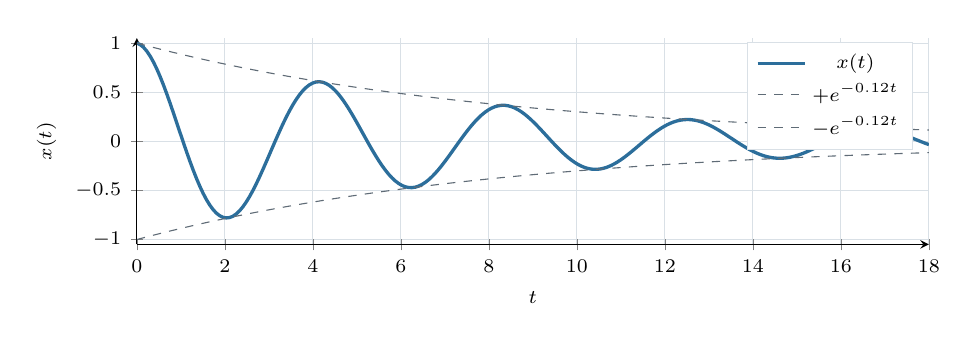
\begin{tikzpicture}
\begin{axis}[
  width=0.96\linewidth,
  height=4.2cm,
  xmin=0,xmax=18,
  ymin=-1.05,ymax=1.05,
  axis lines=left,
  xlabel={$t$},
  ylabel={$x(t)$},
  label style={font=\scriptsize},
  tick label style={font=\scriptsize},
  grid=both,
  major grid style={draw=Line},
  minor grid style={draw=Line!55},
  legend style={
    font=\scriptsize,
    at={(0.98,0.98)},
    anchor=north east,
    draw=Line,
    fill=White
  }
]

\addplot[
  very thick,
  Blue,
  samples=240,
  domain=0:18
]
{exp(-0.12*x)*cos(deg(1.5*x))};

\addplot[
  dashed,
  Slate,
  samples=180,
  domain=0:18
]
{exp(-0.12*x)};

\addplot[
  dashed,
  Slate,
  samples=180,
  domain=0:18
]
{-exp(-0.12*x)};

\legend{$x(t)$,$+e^{-0.12t}$,$-e^{-0.12t}$}
\end{axis}
\end{tikzpicture}
\end{center}

\small\textcolor{Slate}{Vector-style mathematical visualization generated directly in \LaTeX\ using TikZ/Pgfplots.}

\vfill
{\scriptsize\textcolor{Slate}{Consistent fonts, mathematical labels, axes, legends, and reusable figure code.}}
\end{minipage}}
\end{minipage}

\vspace{0.5em}

\section{Structured Tables and Presentation}

\begin{center}
\renewcommand{\arraystretch}{1.22}
\begin{tabularx}{0.98\linewidth}{@{}>{\bfseries\color{Navy}}X>{\centering\arraybackslash}p{2.0cm}>{\centering\arraybackslash}p{2.0cm}>{\centering\arraybackslash}p{2.0cm}@{}}
\toprule
Method & Order & Step Size & Iterations\\
\midrule
\textcolor{Ink}{Explicit Euler} & 1 & 0.010 & 2000\\
\textcolor{Ink}{Midpoint Method} & 2 & 0.010 & 2000\\
\textcolor{Ink}{Classical RK4} & 4 & 0.010 & 2000\\
\bottomrule
\end{tabularx}
\end{center}

\vspace{-0.1em}
{\scriptsize\textcolor{Slate}{Illustrative values shown solely to demonstrate professional table formatting; not reported experimental results.}}

\vspace{0.45em}

\begin{tabularx}{\linewidth}{@{}X@{\hspace{0.4em}}X@{}}
\fcolorbox{Line}{Sky}{%
\begin{minipage}[t][3.25cm][t]{0.92\linewidth}
\miniheader{03 / DOCUMENT STRUCTURE}
\vspace{0.25em}
\bulletline{Automatic equation, table, and figure references}
\bulletline{Consistent heading hierarchy}
\bulletline{Caption and spacing control}
\bulletline{Maintainable section structure}
\bulletline{Clean PDF compilation}
\end{minipage}}
&
\fcolorbox{Line}{Paper}{%
\begin{minipage}[t][3.25cm][t]{0.92\linewidth}
\miniheader{04 / CLIENT WORKFLOW}
\vspace{0.25em}
\bulletline{Review source material and requirements}
\bulletline{Structure content and formatting rules}
\bulletline{Typeset and refine the document}
\bulletline{Quality-check layout and references}
\bulletline{Deliver PDF and editable source}
\end{minipage}}
\end{tabularx}

\vspace{0.38em}

\begin{center}
\pill{MATHEMATICAL FORMATTING}
\hspace{0.15em}\pill{FIGURE DESIGN}
\hspace{0.15em}\pill{TABLE DESIGN}
\hspace{0.15em}\pill{DOCUMENT STRUCTURE}
\hspace{0.15em}\pill{EDITABLE SOURCE}
\end{center}

\vfill

\smallrule
\vspace{0.25em}
\begin{center}
{\footnotesize\bfseries\textcolor{Navy}{LaTeX Typesetting \& Academic/Technical Document Formatting}}\\[-0.1em]
{\scriptsize\textcolor{Slate}{Hammad Hashmi \textbar\ hashmi\_labs \quad | \quad Self-created portfolio sample}}
\end{center}

\end{document}
